\section{二聚体}

依 [11]，本节对边带权的二部图定义二聚体配分函数。我们证明：某些图上的配分函数可以计算为某个小矩阵（其大小与顶点数有关）的子式。然后定义谱簇，并描述由环面上某些二部图构造的 GK 可积系统。

\subsection{二聚体的回顾}

设 $\Gamma$ 是图，记 $E_\Gamma$ 与 $V_\Gamma$ 分别为其边集与顶点集。$\Gamma$ 上的\emph{二聚体构型}是子集 $D\subset E_\Gamma$，使得每个顶点恰含于 $D$ 的一条边中。记 $\mathcal{D}_\Gamma$ 为 $\Gamma$ 上全部二聚体构型的集合，并假定它非空。固定函数 $A: e\mapsto A_e$，它给每条边 $e\in E_\Gamma$ 联系一个复数，称为该边的\emph{权}。

考虑全部二聚体构型之和
\begin{equation}\label{eq:1.25}
S_\Gamma(A)=\sum_{D\in\mathcal{D}_\Gamma}\prod_{e\in D}A_e,
\tag{1.25}
\end{equation}
称之为图 $\Gamma$ 的\emph{二聚体配分函数}。这个配分函数是权变量 $A_e$ 的整系数多项式。

对所谓\emph{开图}，可以把这个构造稍作推广：允许有\emph{终止边}，它带一个特殊的一价顶点，也称为\emph{终止顶点}。没有终止边的图称为\emph{闭图}。两个终止顶点可以等同起来，再删去所得的二价顶点——这样就把两个图粘合起来；反之，可以剪开一条边，宣布新出现的顶点为终止顶点。

开图上的二聚体构型是边的集合，它包含每个内顶点恰一次，对终止边不加任何条件。记 $T_\Gamma$ 为图的终止边集合。对每个子集 $T\subset T_\Gamma$，记 $\mathcal{D}_\Gamma(T)$ 为这样的二聚体构型集合：取自 $T$ 的终止边被占据，其余终止边自由。可以定义\emph{带边界的配分函数}
\begin{equation}\label{eq:1.26}
S_\Gamma(A,T)=\sum_{D\in\mathcal{D}_\Gamma(T)}\prod_{e\in D}A_e.
\tag{1.26}
\end{equation}
所有这些配分函数可以合并成一个\emph{生成配分函数}。固定终止边的次序，并引入奇变量 $\xi=\{\xi_t\mid t\in T_\Gamma\}$。然后定义
\[
S_\Gamma(A,\xi)=\sum_{T\subset T_\Gamma}S_\Gamma(A,T)\prod_{t\in D\cap T}\xi_t,
\]
其中乘积按终止边的固定次序取。

这个生成函数特别方便，因为它在粘合终止边时行为良好。设图 $\Gamma'$ 由 $\Gamma$ 把权为 $A_i$ 的终止边 $i$ 与相邻边 $j$ 粘合而成，其中 $j$ 按所选次序紧随 $i$，权为 $A_j$。所得的边 $e$ 的权为 $A_e=A_iA_j$。

\begin{lemma}\label{lem:1.5.1}
$S_{\Gamma'}(A',\xi')=\int S_\Gamma(A,\xi)e^{\xi_i\xi_j}\,d\xi_j\,d\xi_i$。
\end{lemma}

这里 $\xi'$ 表示去掉 $\xi_i$ 与 $\xi_j$ 后的集合，而 $A'$ 表示把权 $A_e=A_iA_j$ 替换 $A_i$ 与 $A_j$ 后所得的权集合。该引理的证明是显然的，因为
\[
\int S_\Gamma(A,\xi)e^{\xi_i\xi_j}d\xi_j\,d\xi_i=\int S_\Gamma(A,\xi)\,d\xi_j\,d\xi_i+\int S_\Gamma(A,\xi)\xi_i\xi_j\,d\xi_j\,d\xi_i.
\]
右端第一项给出两条终止边 $i$ 与 $j$ 都被占据的二聚体构型之和，它们与图 $\Gamma'$ 中边 $e$ 被占据的二聚体构型一一对应。类似地，第二项给出边 $e$ 为空的构型之和。

\subsection{圆盘上的矩阵与二聚体}

现在证明：对任意矩阵，可以联系一个带终止边与权的二部图，使其配分函数是矩阵子式的生成函数。矩阵乘法对应于粘合图。设 $M$ 为 $n\times n$ 矩阵，$\xi=(\xi_1,\dots,\xi_n)$ 与 $\eta=(\eta_1,\dots,\eta_n)$ 为两组 Grassmann 变量。定义\emph{子式生成函数}
\begin{equation}\label{eq:1.27}
S(M,\xi,\eta)=\exp\Big(\sum_{i,j}M^i_j\xi_i\eta^j\Big).
\tag{1.27}
\end{equation}

\begin{lemma}\label{lem:1.5.2}
函数 (1.27) 满足
\begin{enumerate}[label=(\roman*), leftmargin=2.2em, itemsep=0.15em]
\item $S(M_1M_2,\xi',\eta')=\int S(M_1,\xi',\eta)S(M_2,\xi,\eta')\prod_i\exp(-\xi_i\eta_i)\,d\xi_i\,d\eta_i$；
\item $S(M,\xi,\eta)=1+\sum_{k=1}^n\sum_{\substack{i_1<\dots<i_k\\ j_1<\dots<j_k}}M^{i_1,\dots,i_k}_{j_1,\dots,j_k}\xi_{i_1}\cdots\xi_{i_k}\eta_{j_k}\cdots\eta_{j_1}$；
\item $\int S(M,\xi,\eta)\exp(\mu\sum\eta_i\xi_i)\prod_i d\xi_i\,d\eta_i=\det(\mu-M)$；
\item $\sum_i\Big(\xi_i\frac{\partial}{\partial\tilde\xi_i}-\tilde\eta_i\frac{\partial}{\partial\eta_i}\Big)S(M,\xi,\eta)S(M,\tilde\xi,\tilde\eta)=0$。
\end{enumerate}
\end{lemma}

这里 $M^{i_1,\dots,i_k}_{j_1,\dots,j_k}$ 表示矩阵 $M$ 对应于行 $i_1<\dots<i_k$ 与列 $j_1<\dots<j_k$ 的子式。引理 1.5.2 表明，函数 $S(M,\xi,\eta)$ 可以看作矩阵 $M$ 的全部子式的生成函数。它等价于子式的 Plücker 关系。该引理的证明见附录 1.13。

现在容易建立下述结果。

\begin{lemma}\label{lem:1.5.3}
对任意矩阵 $M$ 都可以构造一个带有序边与边权的平面二部图 $\Gamma_M$，使得它的子式生成函数 $S(M,\xi,\eta)$ 与图的生成配分函数 $S_{\Gamma_M}(A,\xi,\eta)$ 相同。
\end{lemma}

事实上，比较引理 1.5.2 与 1.5.1 可见，粘合图对应于矩阵乘法。因此只需对 $\operatorname{GL}(N)$ 的一组生成元验证带权图的存在，即对对角矩阵与指数化的单根 (1.7)。列举全部二聚体构型即可验证：图 1.6 中的图分别对应于矩阵 $H_a=\operatorname{diag}(a_1,\dots,a_N)$、$E_i$ 与 $E_{\bar\imath}$，子式生成函数分别为 $S(H_a,\xi,\eta)=\exp(\sum_j a_j\xi_j\eta_j)$、$S(E_i,\xi,\eta)=\exp(\xi_i\eta_{i+1}+\sum_j\xi_j\eta_j)$ 与 $S(E_{\bar\imath},\xi,\eta)=\exp(\xi_{i+1}\eta_i+\sum_j\xi_j\eta_j)$。我们假定图的终止边按逆时针排序：先左侧自上而下（$\xi$ 变量），再右侧自下而上（$\eta$ 变量）。

\begin{figure}[htbp]
\centering
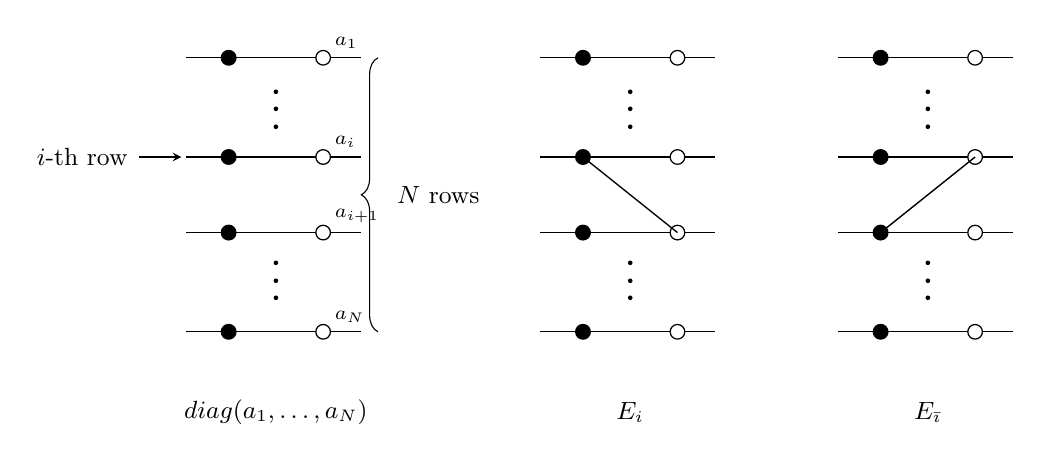
\begin{tikzpicture}[scale=1.20]
\draw[line width=0.5pt] (-0.45,3.00) -- (0.00,3.00);
\draw[line width=0.5pt] (0.00,3.00) -- (1.00,3.00);
\draw[line width=0.5pt] (1.00,3.00) -- (1.40,3.00);
\fill (0.00,3.00) circle (2.4pt);
\fill[white] (1.00,3.00) circle (2.2pt);
\draw[line width=0.45pt] (1.00,3.00) circle (2.2pt);
\node[font=\scriptsize,above right] at (1.02,3.00) {$a_1$};
\draw[line width=0.5pt] (-0.45,1.95) -- (0.00,1.95);
\draw[line width=0.5pt] (0.00,1.95) -- (1.00,1.95);
\draw[line width=0.5pt] (1.00,1.95) -- (1.40,1.95);
\fill (0.00,1.95) circle (2.4pt);
\fill[white] (1.00,1.95) circle (2.2pt);
\draw[line width=0.45pt] (1.00,1.95) circle (2.2pt);
\node[font=\scriptsize,above right] at (1.02,1.95) {$a_i$};
\draw[line width=0.5pt] (-0.45,1.15) -- (0.00,1.15);
\draw[line width=0.5pt] (0.00,1.15) -- (1.00,1.15);
\draw[line width=0.5pt] (1.00,1.15) -- (1.40,1.15);
\fill (0.00,1.15) circle (2.4pt);
\fill[white] (1.00,1.15) circle (2.2pt);
\draw[line width=0.45pt] (1.00,1.15) circle (2.2pt);
\node[font=\scriptsize,above right] at (1.02,1.15) {$a_{i+1}$};
\draw[line width=0.5pt] (-0.45,0.10) -- (0.00,0.10);
\draw[line width=0.5pt] (0.00,0.10) -- (1.00,0.10);
\draw[line width=0.5pt] (1.00,0.10) -- (1.40,0.10);
\fill (0.00,0.10) circle (2.4pt);
\fill[white] (1.00,0.10) circle (2.2pt);
\draw[line width=0.45pt] (1.00,0.10) circle (2.2pt);
\node[font=\scriptsize,above right] at (1.02,0.10) {$a_N$};
\fill (0.50,2.64) circle (0.7pt);
\fill (0.50,2.46) circle (0.7pt);
\fill (0.50,2.27) circle (0.7pt);
\fill (0.50,0.83) circle (0.7pt);
\fill (0.50,0.64) circle (0.7pt);
\fill (0.50,0.46) circle (0.7pt);
\draw[decorate,decoration={brace,amplitude=6pt},line width=0.4pt] (1.58,0.10) -- (1.58,3.00);\node[font=\small,right] at (1.68,1.55) {$N$ rows};\node[font=\small] at (-1.55,1.95) {$i$-th row};\draw[line width=0.4pt,->,>=stealth] (-0.95,1.95) -- (-0.50,1.95);
\node[font=\small] at (0.50,-0.75) {$\operatorname{diag}(a_1,\dots,a_N)$};
\begin{scope}[xshift=3.75cm]
\draw[line width=0.5pt] (-0.45,3.00) -- (0.00,3.00);
\draw[line width=0.5pt] (0.00,3.00) -- (1.00,3.00);
\draw[line width=0.5pt] (1.00,3.00) -- (1.40,3.00);
\fill (0.00,3.00) circle (2.4pt);
\fill[white] (1.00,3.00) circle (2.2pt);
\draw[line width=0.45pt] (1.00,3.00) circle (2.2pt);
\draw[line width=0.5pt] (-0.45,1.95) -- (0.00,1.95);
\draw[line width=0.5pt] (0.00,1.95) -- (1.00,1.95);
\draw[line width=0.5pt] (1.00,1.95) -- (1.40,1.95);
\fill (0.00,1.95) circle (2.4pt);
\fill[white] (1.00,1.95) circle (2.2pt);
\draw[line width=0.45pt] (1.00,1.95) circle (2.2pt);
\draw[line width=0.5pt] (-0.45,1.15) -- (0.00,1.15);
\draw[line width=0.5pt] (0.00,1.15) -- (1.00,1.15);
\draw[line width=0.5pt] (1.00,1.15) -- (1.40,1.15);
\fill (0.00,1.15) circle (2.4pt);
\fill[white] (1.00,1.15) circle (2.2pt);
\draw[line width=0.45pt] (1.00,1.15) circle (2.2pt);
\draw[line width=0.5pt] (-0.45,0.10) -- (0.00,0.10);
\draw[line width=0.5pt] (0.00,0.10) -- (1.00,0.10);
\draw[line width=0.5pt] (1.00,0.10) -- (1.40,0.10);
\fill (0.00,0.10) circle (2.4pt);
\fill[white] (1.00,0.10) circle (2.2pt);
\draw[line width=0.45pt] (1.00,0.10) circle (2.2pt);
\fill (0.50,2.64) circle (0.7pt);
\fill (0.50,2.46) circle (0.7pt);
\fill (0.50,2.27) circle (0.7pt);
\fill (0.50,0.83) circle (0.7pt);
\fill (0.50,0.64) circle (0.7pt);
\fill (0.50,0.46) circle (0.7pt);
\draw[line width=0.5pt] (0.00,1.95) -- (1.00,1.15);
\node[font=\small] at (0.50,-0.75) {$E_i$};
\end{scope}
\begin{scope}[xshift=6.90cm]
\draw[line width=0.5pt] (-0.45,3.00) -- (0.00,3.00);
\draw[line width=0.5pt] (0.00,3.00) -- (1.00,3.00);
\draw[line width=0.5pt] (1.00,3.00) -- (1.40,3.00);
\fill (0.00,3.00) circle (2.4pt);
\fill[white] (1.00,3.00) circle (2.2pt);
\draw[line width=0.45pt] (1.00,3.00) circle (2.2pt);
\draw[line width=0.5pt] (-0.45,1.95) -- (0.00,1.95);
\draw[line width=0.5pt] (0.00,1.95) -- (1.00,1.95);
\draw[line width=0.5pt] (1.00,1.95) -- (1.40,1.95);
\fill (0.00,1.95) circle (2.4pt);
\fill[white] (1.00,1.95) circle (2.2pt);
\draw[line width=0.45pt] (1.00,1.95) circle (2.2pt);
\draw[line width=0.5pt] (-0.45,1.15) -- (0.00,1.15);
\draw[line width=0.5pt] (0.00,1.15) -- (1.00,1.15);
\draw[line width=0.5pt] (1.00,1.15) -- (1.40,1.15);
\fill (0.00,1.15) circle (2.4pt);
\fill[white] (1.00,1.15) circle (2.2pt);
\draw[line width=0.45pt] (1.00,1.15) circle (2.2pt);
\draw[line width=0.5pt] (-0.45,0.10) -- (0.00,0.10);
\draw[line width=0.5pt] (0.00,0.10) -- (1.00,0.10);
\draw[line width=0.5pt] (1.00,0.10) -- (1.40,0.10);
\fill (0.00,0.10) circle (2.4pt);
\fill[white] (1.00,0.10) circle (2.2pt);
\draw[line width=0.45pt] (1.00,0.10) circle (2.2pt);
\fill (0.50,2.64) circle (0.7pt);
\fill (0.50,2.46) circle (0.7pt);
\fill (0.50,2.27) circle (0.7pt);
\fill (0.50,0.83) circle (0.7pt);
\fill (0.50,0.64) circle (0.7pt);
\fill (0.50,0.46) circle (0.7pt);
\draw[line width=0.5pt] (0.00,1.15) -- (1.00,1.95);
\node[font=\small] at (0.50,-0.75) {$E_{\bar\imath}$};
\end{scope}
\end{tikzpicture}
\caption{对应于 $\operatorname{GL}(N)$ 的生成元的图。权变量 $a$ 全部赋给终止边（在我们的选择中，即右侧那些与 $\eta$-变量相联系的终止边）。其余所有权都等于 $1$。}
\label{fig:1.6}
\end{figure}

\subsection{带符号的二聚体配分函数}

不幸的是，这个简单配方无法以统一的方式构造对应于仿射群 $\widehat{\operatorname{PGL}}(N)$ 的生成元 (1.18)、(1.19) 的图。可以用简单得多的办法做到这一点：给二聚体构型赋符号；特别地，给出一个对整数 $N$ 与奇数 $N$ 两种情形都适用于群 $\widehat{\operatorname{PGL}}(N)$ 的算法。此外，这是解释 (1.23) 中出现不同符号项的最直接方式，下面将把它与某些二聚体配分函数作比较。从现在起假定图 $\Gamma$ 嵌入曲面 $\Sigma$，终止顶点（若有）在 $\Sigma$ 的边界上。

任何二聚体构型都可视为链空间 $C_1(\Gamma,\Z/2\Z)$ 的元素。固定元素 $Q\in Z_1(\Sigma,\Z/2\Z)\otimes Z_1(\Sigma,\partial\Sigma,\Z/2\Z)$，使其到同调的投影给出 $H_1(\Sigma,\Z/2\Z)\otimes H_1(\Sigma,\partial\Sigma,\Z/2\Z)$ 中的典范元。这样的 $Q$ 可解释为 $C_1(\Gamma,\Z/2\Z)$ 上的二次型，特别地也是其由二聚体构型张成的子空间上的二次型。任意两个这样的型之差是线性型。为构造这样的型，可以选取代表 $H_1(\Sigma,\Z/2\Z)$ 的一组基的圈族 $\{\alpha_i\}$，以及代表 $H_1(\Sigma,\partial\Sigma,\Z/2\Z)$ 中对偶基的圈族 $\{\beta_i\}$。则型由 $Q=\sum_i\alpha_i\otimes\beta_i$ 给出，它在二聚体构型 $D$ 上的值等于
\[
Q(D)=\sum_i\langle\alpha_i,D\rangle\langle\beta_i,D\rangle.
\]
用这个二次型可以把 (1.25) 修改为
\begin{equation}\label{eq:1.28}
S_{\Gamma,Q}(A)=\sum_{D\in\mathcal{D}_\Gamma}(-1)^{Q(D)}\prod_{e\in D}A_e,
\tag{1.28}
\end{equation}
并把 (1.26) 修改为
\[
S_{\Gamma,Q}(A,T)=\sum_{D\in\mathcal{D}_\Gamma(T)}(-1)^{Q(D)}\prod_{e\in D}A_e.
\]

用闭曲线剪开带型 $Q$ 的曲面 $\Sigma$，在所得曲面 $\Sigma'$ 上诱导一个型 $Q'$。型 $Q'$ 由下述条件定义：对 $\Gamma\subset\Sigma$ 上的任意二聚体构型 $D$，有 $Q(D)=Q(D')$，其中 $D'$ 是剪开构型 $D$ 所得的构型。此时称 $Q$ 与 $Q'$ \emph{相容}。

在图中，我们把余圈 $\alpha_i\in Z_1(\Sigma,\Z/2\Z)$ 与 $\beta_i\in Z_1(\Sigma,\partial\Sigma,\Z/2\Z)$ 画成曲面上横截于图 $\Gamma$ 的相应圈。前者用可以从边界到边界的圈表示，后者用闭圈表示。

\subsection{柱面上的 $\widehat{\operatorname{PGL}}(N)$ 与二聚体}

本节把仿射群 $\widehat{\operatorname{PGL}}(N)\subset\operatorname{PGL}^{\sharp}(N)$ 的元素表示成带符号的二聚体配分函数。$\operatorname{PGL}^{\sharp}(N)$ 的生成元 (1.17)、(1.18) 的乘积属于 $\widehat{\operatorname{PGL}}(N)$，当且仅当条件 (1.22) 满足。

生成元 (1.17) 对应的图与图 1.6 中相同，只是现在嵌入短的横柱面，如图 1.7。对这些矩阵，公式 (1.26) 与 (1.28) 给出相同结果，只要按图选取圈 $\alpha$ 与 $\beta$：因为圈 $\beta$ 从边界到边界且不与图相交，故 $Q(D)=\langle\alpha,D\rangle\langle\beta,D\rangle=0$，所有二聚体构型的符号都是正的。

$\widehat{\operatorname{PGL}}(N)$ 特有的生成元 (1.18)、(1.19) 可由图 1.8 中嵌入柱面的图表示。所有生成元 (1.18)、(1.19) 只有一个非零矩阵元，等于 $\lambda^{\pm1}$，位于主对角线、上次对角线与下次对角线之外。因此，按子式生成函数 (1.27) 对矩阵 $E_0(\lambda)$、$E_{\bar0}(\lambda)$ 与 $\Lambda(\lambda)$ 的展开，所有 $\lambda$-相关子式依其大小 $k=1,\dots,N$ 对奇数（偶数）$k$ 分别取正（负）号。顾及这些符号的最简单办法是：(i) 对图中对应于 $\lambda$-相关矩阵元的每条链赋予权 $-\lambda$（而不是朴素的 $+\lambda$）；(ii) 按规则 (1.28) 给所有二聚体构型赋符号。

容易看出，沿边界圆粘合柱面与二次型 $Q=\alpha\otimes\beta$ 相容，其中 $\beta$ 是柱面的水平生成元，$\alpha$ 是它在某个边界附近小邻域中的竖直截线。注意这样的型 $Q$ 与圈 $\alpha$ 的两种可能选择无关（因为它们之间的顶点数为偶），并且这个型与把两个柱面粘合相容。

\begin{figure}[htbp]
\centering
\begin{tikzpicture}[scale=1.20]
\draw[line width=0.5pt] (-0.45,3.00) -- (0.00,3.00);
\draw[line width=0.5pt] (0.00,3.00) -- (1.00,3.00);
\draw[line width=0.5pt] (1.00,3.00) -- (1.40,3.00);
\fill (0.00,3.00) circle (2.4pt);
\fill[white] (1.00,3.00) circle (2.2pt);
\draw[line width=0.45pt] (1.00,3.00) circle (2.2pt);
\node[font=\scriptsize,above right] at (1.02,3.00) {$a_1$};
\draw[line width=0.5pt] (-0.45,1.95) -- (0.00,1.95);
\draw[line width=0.5pt] (0.00,1.95) -- (1.00,1.95);
\draw[line width=0.5pt] (1.00,1.95) -- (1.40,1.95);
\fill (0.00,1.95) circle (2.4pt);
\fill[white] (1.00,1.95) circle (2.2pt);
\draw[line width=0.45pt] (1.00,1.95) circle (2.2pt);
\node[font=\scriptsize,above right] at (1.02,1.95) {$a_i$};
\draw[line width=0.5pt] (-0.45,1.15) -- (0.00,1.15);
\draw[line width=0.5pt] (0.00,1.15) -- (1.00,1.15);
\draw[line width=0.5pt] (1.00,1.15) -- (1.40,1.15);
\fill (0.00,1.15) circle (2.4pt);
\fill[white] (1.00,1.15) circle (2.2pt);
\draw[line width=0.45pt] (1.00,1.15) circle (2.2pt);
\node[font=\scriptsize,above right] at (1.02,1.15) {$a_{i+1}$};
\draw[line width=0.5pt] (-0.45,0.10) -- (0.00,0.10);
\draw[line width=0.5pt] (0.00,0.10) -- (1.00,0.10);
\draw[line width=0.5pt] (1.00,0.10) -- (1.40,0.10);
\fill (0.00,0.10) circle (2.4pt);
\fill[white] (1.00,0.10) circle (2.2pt);
\draw[line width=0.45pt] (1.00,0.10) circle (2.2pt);
\node[font=\scriptsize,above right] at (1.02,0.10) {$a_N$};
\fill (0.50,2.64) circle (0.7pt);
\fill (0.50,2.46) circle (0.7pt);
\fill (0.50,2.27) circle (0.7pt);
\fill (0.50,0.83) circle (0.7pt);
\fill (0.50,0.64) circle (0.7pt);
\fill (0.50,0.46) circle (0.7pt);
\draw[dashed,line width=0.4pt] (0.50,-0.45) -- (0.50,3.45);
\node[font=\scriptsize,above] at (0.62,3.45) {$\alpha$};
\draw[dashed,line width=0.4pt] (-0.55,-0.28) -- (1.55,-0.28);
\node[font=\scriptsize,right] at (1.55,-0.28) {$\beta$};
\node[font=\small] at (0.50,-0.95) {$\operatorname{diag}(a_1,\dots,a_N)$};
\begin{scope}[xshift=3.75cm]
\draw[line width=0.5pt] (-0.45,3.00) -- (0.00,3.00);
\draw[line width=0.5pt] (0.00,3.00) -- (1.00,3.00);
\draw[line width=0.5pt] (1.00,3.00) -- (1.40,3.00);
\fill (0.00,3.00) circle (2.4pt);
\fill[white] (1.00,3.00) circle (2.2pt);
\draw[line width=0.45pt] (1.00,3.00) circle (2.2pt);
\draw[line width=0.5pt] (-0.45,1.95) -- (0.00,1.95);
\draw[line width=0.5pt] (0.00,1.95) -- (1.00,1.95);
\draw[line width=0.5pt] (1.00,1.95) -- (1.40,1.95);
\fill (0.00,1.95) circle (2.4pt);
\fill[white] (1.00,1.95) circle (2.2pt);
\draw[line width=0.45pt] (1.00,1.95) circle (2.2pt);
\draw[line width=0.5pt] (-0.45,1.15) -- (0.00,1.15);
\draw[line width=0.5pt] (0.00,1.15) -- (1.00,1.15);
\draw[line width=0.5pt] (1.00,1.15) -- (1.40,1.15);
\fill (0.00,1.15) circle (2.4pt);
\fill[white] (1.00,1.15) circle (2.2pt);
\draw[line width=0.45pt] (1.00,1.15) circle (2.2pt);
\draw[line width=0.5pt] (-0.45,0.10) -- (0.00,0.10);
\draw[line width=0.5pt] (0.00,0.10) -- (1.00,0.10);
\draw[line width=0.5pt] (1.00,0.10) -- (1.40,0.10);
\fill (0.00,0.10) circle (2.4pt);
\fill[white] (1.00,0.10) circle (2.2pt);
\draw[line width=0.45pt] (1.00,0.10) circle (2.2pt);
\fill (0.50,2.64) circle (0.7pt);
\fill (0.50,2.46) circle (0.7pt);
\fill (0.50,2.27) circle (0.7pt);
\fill (0.50,0.83) circle (0.7pt);
\fill (0.50,0.64) circle (0.7pt);
\fill (0.50,0.46) circle (0.7pt);
\draw[dashed,line width=0.4pt] (0.50,-0.45) -- (0.50,3.45);
\node[font=\scriptsize,above] at (0.62,3.45) {$\alpha$};
\draw[dashed,line width=0.4pt] (-0.55,-0.28) -- (1.55,-0.28);
\node[font=\scriptsize,right] at (1.55,-0.28) {$\beta$};
\node[font=\small] at (0.50,-0.95) {$E_i$};
\end{scope}
\begin{scope}[xshift=6.90cm]
\draw[line width=0.5pt] (-0.45,3.00) -- (0.00,3.00);
\draw[line width=0.5pt] (0.00,3.00) -- (1.00,3.00);
\draw[line width=0.5pt] (1.00,3.00) -- (1.40,3.00);
\fill (0.00,3.00) circle (2.4pt);
\fill[white] (1.00,3.00) circle (2.2pt);
\draw[line width=0.45pt] (1.00,3.00) circle (2.2pt);
\draw[line width=0.5pt] (-0.45,1.95) -- (0.00,1.95);
\draw[line width=0.5pt] (0.00,1.95) -- (1.00,1.95);
\draw[line width=0.5pt] (1.00,1.95) -- (1.40,1.95);
\fill (0.00,1.95) circle (2.4pt);
\fill[white] (1.00,1.95) circle (2.2pt);
\draw[line width=0.45pt] (1.00,1.95) circle (2.2pt);
\draw[line width=0.5pt] (-0.45,1.15) -- (0.00,1.15);
\draw[line width=0.5pt] (0.00,1.15) -- (1.00,1.15);
\draw[line width=0.5pt] (1.00,1.15) -- (1.40,1.15);
\fill (0.00,1.15) circle (2.4pt);
\fill[white] (1.00,1.15) circle (2.2pt);
\draw[line width=0.45pt] (1.00,1.15) circle (2.2pt);
\draw[line width=0.5pt] (-0.45,0.10) -- (0.00,0.10);
\draw[line width=0.5pt] (0.00,0.10) -- (1.00,0.10);
\draw[line width=0.5pt] (1.00,0.10) -- (1.40,0.10);
\fill (0.00,0.10) circle (2.4pt);
\fill[white] (1.00,0.10) circle (2.2pt);
\draw[line width=0.45pt] (1.00,0.10) circle (2.2pt);
\fill (0.50,2.64) circle (0.7pt);
\fill (0.50,2.46) circle (0.7pt);
\fill (0.50,2.27) circle (0.7pt);
\fill (0.50,0.83) circle (0.7pt);
\fill (0.50,0.64) circle (0.7pt);
\fill (0.50,0.46) circle (0.7pt);
\draw[dashed,line width=0.4pt] (0.50,-0.45) -- (0.50,3.45);
\node[font=\scriptsize,above] at (0.62,3.45) {$\alpha$};
\draw[dashed,line width=0.4pt] (-0.55,-0.28) -- (1.55,-0.28);
\node[font=\scriptsize,right] at (1.55,-0.28) {$\beta$};
\node[font=\small] at (0.50,-0.95) {$E_{\bar\imath}$};
\end{scope}
\end{tikzpicture}
\caption{柱面上的图，对应于 $\operatorname{PGL}(N)$ 与 $\widehat{\operatorname{PGL}}(N)$ 的公共生成元。圈 $\alpha\in H_1(\Sigma,\Z/2\Z)$ 用绕过柱面的竖直虚线表示，而圈 $\beta\in H_1(\Sigma,\partial\Sigma,\Z/2\Z)$ 对应水平虚线，在柱面的背面连接它的两条边界。}
\label{fig:1.7}
\end{figure}

\subsection{二聚体与离散 Dirac 算子}

现在证明：对闭曲面，带符号的配分函数 (1.28) 等于一个矩阵的行列式，该矩阵称为\emph{离散 Dirac 算子}。为定义这个算子，首先要固定曲面的自旋结构（即便固定了，行列式也只定义到符号）。然而对自旋结构的依赖并不本质，配分函数的等价类不依赖于此选择。这一构造主要归功于 P. Kasteleyn [16]，并由 D. Cimasoni 与 N. Reshetikhin [2] 推广到高亏格。

回忆：闭曲面上的自旋结构可以等同于 $H_1(\Sigma,\Z/2\Z)$ 上与相交指数 $\langle\cdot,\cdot\rangle$ 满足相容条件的二次型 [14]：
\begin{equation}\label{eq:1.29}
Q(x+y)+Q(x)+Q(y)=\langle x,y\rangle\quad(\mathrm{mod}\ 2).
\tag{1.29}
\end{equation}
曲面上的自旋结构可以用二部图边的 \emph{Kasteleyn 标号}来编码。嵌入曲面 $\Sigma$ 的图 $\Gamma$ 的 Kasteleyn 标号，是用数 $K=K_e\in\{\pm1\}$ 对 $\Gamma$ 的边所作的标号，使得对任何有 $l(f)$ 条边的面 $f$，沿其边界的 $K_e$ 之积等于 $(-1)^{l(f)/2+1}$（即绕边数为 $4$ 的倍数的面单值为 $-1$，其余为 $+1$）。这种标号可视为上链 $K\in C^1(\Gamma,\{\pm1\})$，满足条件 $\partial K=R$，其中 $R$ 是在面 $f$ 上取值 $(-1)^{l/2+1}$ 的余圈。

给定两个二聚体构型 $D_1$ 与 $D_2$，可以定义它们的\emph{互 parity} $\sigma(D_1,D_2)\in\{\pm1\}$ 如下。每个二聚体构型 $D$ 定义映射（仍记作 $D$）：$B\to W$，从黑顶点集到白顶点集。parity $\sigma(D_1,D_2)$ 就是映射 $(D_1-D_2): W\to W$ 的奇偶性；显然对任意三个二聚体构型 $D_1$、$D_2$、$D_3$ 有 $\sigma(D_1,D_2)\sigma(D_2,D_3)\sigma(D_3,D_1)=1$。下述引理的证明基本包含在 [2] 中。

\begin{lemma}\label{lem:1.5.4}
\begin{enumerate}[label=(\roman*), leftmargin=2.2em, itemsep=0.15em]
\item Kasteleyn 标号存在，且唯一到 $Z^1(\Gamma,\{\pm1\})$ 中的上链；
\item 对任意 Kasteleyn 标号 $K$ 与任意满足 $D_1-D_0\in B_1(\Sigma,\Z/2\Z)$ 的二聚体构型 $D_0$、$D_1$，有 $\sigma(D_1,D_0)\langle(D_1-D_0),K\rangle=1$；
\item 对任意 Kasteleyn 标号与任意满足 $D_0+D_1+D_2+D_3\in B_1(\Sigma,\Z/2\Z)$ 的四个二聚体构型 $D_0$、$D_1$、$D_2$、$D_3$，有
\[
\sigma(D_1,D_2)\sigma(D_0,D_3)\langle(D_1-D_0),(D_2-D_0)\rangle\langle(D_0+D_1+D_2+D_3),K\rangle=1.
\]
\end{enumerate}
\end{lemma}

\begin{corollary}\label{cor:1.5.5}
固定二聚体构型 $D_0$，考虑二聚体构型集合上的函数 $q:\mathcal{D}_\Gamma\to\{\pm1\}$，定义为 $q(D)=\langle(D-D_0),K\rangle\sigma(D,D_0)$。引理 1.5.4(ii) 蕴涵 $q(D_0)=1$ 且其值只依赖 $D-D_0$ 的同调类，而引理 1.5.4(iii) 等价于把它写成
\[
q(D)=(-1)^{Q(D-D_0)},
\]
其中 $Q$ 是表示自旋结构的二次型。
\end{corollary}

定义线性算子 $D(A): C_W\to C_B$ 为
\[
D(A)=\sum_e\langle e,KA\rangle b(e)w(e),
\]
其中 $b(e)$ 是 $\C$ 到对应于边 $e$ 的黑端的因子的嵌入，$w(e)$ 是到对应于白端的因子的投影。换言之，算子 $D(A)$ 的矩阵以黑顶点为行、白顶点为列，白顶点 $w$ 与黑顶点 $b$ 之间的矩阵元等于沿一切连接 $b$ 与 $w$ 的边 $e$ 之和
\[
D(A)_{bw}=\sum_{e:b\to w}K_eA_e.
\]
按上边缘改变 $A$ 与 $K$（作离散规范变换）相当于从两侧乘以 $D(A)$ 的非退化对角矩阵。因此 $D(A)$ 的退化只依赖 $A$ 在 $H^1(\Gamma)$ 中的类。

\begin{lemma}\label{lem:1.5.6}
$\det D(A)=\pm S_\Gamma(A)$。
\end{lemma}

\begin{remark}\label{rem:1.5.7}
尽管 Dirac 算子 $D$ 经由 Kasteleyn 定向 $K$ 依赖于曲面上的自旋结构，这一依赖由简单规则
\[
D_{K'}(A)=D_K(AK'/K)
\]
给出。此式有意义，因为比值 $K'/K$ 可视为 $H^1(\Sigma)$ 的元素（因此我们省略下标 $K$）。
\end{remark}

\begin{proof}
在固定 $C_W$ 与 $C_B$ 上体积形式之间的同构之前，算子 $D(A)$ 的行列式没有定义。选取 $W$ 与 $B$ 之间的双射可建立这样的同构，但不同选择给出不同的行列式符号，因此后者只定义到符号。可以通过选取二聚体构型 $D_0$ 来固定一个双射。一旦固定双射，就可以谈论映射 $s: B\to W$ 的奇偶性 $\operatorname{sign}(s)$，行列式的公式为
\[
\det D(A)=\sum_{s:B\to W}\prod_{b\in B}(-1)^{\operatorname{sign}(s)}D_{b,s(b)},
\]
其中和取遍一切双射 $s: B\to W$。每个二聚体构型 $D$ 定义一个双射（仍记作 $D$），而不对应于二聚体构型的双射对行列式没有贡献。因此行列式的公式可以改写为
\[
\begin{aligned}
\det D(A)&=\sum_{D\in\mathcal{D}_\Gamma}(-1)^{\sigma(D,D_0)}\langle D,KA\rangle\\
&=\langle D_0,K\rangle\sum_{D\in\mathcal{D}_\Gamma}(-1)^{\sigma(D,D_0)}\langle(D-D_0),K\rangle\langle D,A\rangle
=\pm\sum_{D\in\mathcal{D}_\Gamma}(-1)^{Q(D-D_0)}\langle D,A\rangle,
\end{aligned}
\]
其中最后一个等号由推论 1.5.5 成立。
\end{proof}

\subsection{谱子流形与面配分函数}

现在考虑闭曲面 $\Sigma$、其上的二部图 $\Gamma$，以及相应的带符号二聚体配分函数。对边参数 $A$ 的某些取值集合，配分函数为零；由于它是算子 $D(A)$ 的行列式，$D(A)$ 的核在这个集合上构成线丛。然而，在参数空间 $A$ 上有一个很大的规范对称群作用，保持零点集不变。\emph{谱子流形}就是零点集对这个群的商。

我们先用在初等代数拓扑的语言描述全部边参数对规范群的商。

由于二部图的边有典范定向（从白顶点到黑顶点），任何二聚体构型都可解释为 $\Gamma$ 上整系数 1-链空间 $C_1(\Gamma,\Z)$ 的元素。任何二聚体构型的边界只是一个 0-链，即黑顶点之和减去白顶点之和，记作 $v=b-w$。因此任意两个二聚体构型之差是闭链。

边上的权 $A=\{A_e\}$ 可视为 $\Gamma$ 的以乘法群 $\C^\times$ 为系数的 1-上链空间 $C^1(\Gamma,\C^\times)$ 的元素，而乘积 $\prod_{e\in D}A_e=\langle A,D\rangle$ 正是 1-链与 1-上链之间的典范配对。配分函数 (1.28) 的表达式可写成
\[
S_\Gamma(A)=\sum_{D\in\mathcal{D}_\Gamma}(-1)^{Q(D)}\langle A,D\rangle.
\]
下面除非另有说明，我们假定一切整系数链群按加法写（因为它们只是自由有限生成阿贝尔群）；另一方面，一切上链群以 $\C^\times$ 为系数、按乘法考虑（因为它们是代数环面）。

函数 $S_\Gamma(A)$ 关于规范群 $C^0(\Gamma)$ 的作用是齐次的。即 $S_\Gamma(A\partial g)=S_\Gamma(A)\langle g,w-b\rangle$，其中 $b,w\in C^0(\Gamma)$ 分别是黑顶点与白顶点之和。确实，
\[
S_\Gamma(A\partial g)=\sum_{D\in\mathcal{D}_\Gamma}(-1)^{Q(D)}\langle A\partial g,D\rangle
=\sum_{D\in\mathcal{D}_\Gamma}(-1)^{Q(D)}\langle A,D\rangle\langle\partial g,D\rangle
=S_\Gamma(A)\langle g,w-b\rangle.
\]
这意味着配分函数 $S_\Gamma(\cdot)$ 以及任意 $\langle\cdot,D_0\rangle$（$D_0$ 为二聚体构型）都可解释为商 $H^1(\Gamma)=C^1(\Gamma)/\partial C^0(\Gamma)$ 上某个线丛的截面。比值 $S_\Gamma(\cdot)/\langle\cdot,D_0\rangle$ 只是 $H^1(\Gamma)$ 上的函数。这个截面的零点迹就是我们的谱簇 $L$。

注意，由于图嵌入闭曲面 $\Sigma$，有正合列
\begin{equation}\label{eq:1.30}
1\to H^1(\Sigma)\to H^1(\Gamma)\xrightarrow{\ \partial\ }B^2(\Sigma)\to1,
\tag{1.30}
\end{equation}
其中 $B^2(\Sigma)$ 是 2-上边缘群，在我们情形下就是给曲面的面赋以乘积为 $1$ 的非零数的群。这个正合列在 $H^1(\Gamma)$ 上定义了主 $H^1(\Sigma)$-丛的结构。

现在假定 $\Sigma$ 是环面，$M$ 为 $H^1(\Sigma)$ 中平面曲线的模空间，它只是一个二维代数环面，模去 $H^1(\Sigma)$ 元素的（乘法）平移。设平面曲线的\emph{万有 Jacobi 丛} $J$ 为（曲线，其上的线丛）之对的空间，同样模去 $H^1(\Sigma)$ 的作用。

$M$ 的点对应于多项式 $P(\lambda)=\sum_{i\in H^1(\Sigma)}H_i\langle i,\lambda\rangle$，模去变换 $P(\lambda)\to\alpha P(\beta\lambda)$，其中 $\alpha\in\C^\times$、$\beta\in H^1(\Sigma)$。空间 $M$ 与 $J$ 分别按具有给定 Newton 多边形 $\Delta\subset H^1(\Sigma)$ 的曲线分层为有限维子空间 $M_\Delta$ 与 $J_\Delta$。多边形 $\Delta$ 就是使 $H_i\neq0$ 的点 $i\in H^1(\Sigma)$ 的凸包。

Newton 多边形 $\Delta$ 的顶点处的系数 $H_i$ 必须非零。取任意三个顶点，可以把多项式 $F(\lambda)=\sum_{i\in\Delta}H_i(x)\langle i,\lambda\rangle$ 化为在这三个顶点处系数为 $1$ 的法式（我们称之为曲线的\emph{归一化方程}）。其余系数是空间 $M_\Delta$ 上的坐标。

对任意点 $x\in B^2(\Sigma)$，谱簇与 $x$ 上纤维的交是曲线，而 Dirac 算子的核在它上面（只要曲线非奇异）定义线丛。纤维同构于 $H^1(\Sigma)$，但这个同构定义到平移。因此，到曲线模空间的\emph{作用映射} $I: B^2(\Sigma)\to M$，以及到万有 Jacobi 丛的\emph{作用–角映射}（有理映射）$J: B^2(\Sigma)\to J$，都是定义良好的。

正合列蕴涵 $H^1(\Gamma)$ 同构于乘积 $H^1(\Sigma)\times B^2(\Sigma)$，但同构不是典范的。固定这样一个同构，并在离散联络中选取 $H^1(\Gamma)$ 的代表，得到映射 $A: B^2(\Sigma)\times H^1(\Gamma)\to C^1(\Gamma)$。用于在坐标中计算作用映射的\emph{面配分函数}由 $S^f_\Gamma(\lambda,x)=S_\Gamma(A(\lambda,x))$ 给出。换另一个同构时，面配分函数按规则
\begin{equation}\label{eq:1.31}
S^f_\Gamma(\lambda,x)\mapsto\alpha(x)S^f_\Gamma(\beta(x)\lambda,x)
\tag{1.31}
\end{equation}
变化，其中 $\alpha: B^2(\Sigma)\to\C^\times$ 与 $\beta: B^2(\Sigma)\to H^1(\Sigma)$ 是任意同态。

面配分函数
\begin{equation}\label{eq:1.32}
S^f_\Gamma(\lambda,x)=\sum_{i\in\Delta}H_i(x)\langle\lambda,i\rangle
\tag{1.32}
\end{equation}
因而对任意 $x$ 值定义平面曲线模空间 $M$ 的一个点。我们总可以选择使三个顶点系数为 $1$ 的分裂，从而使面配分函数成为归一化的。

注意归一化面配分函数不依赖自旋结构。确实，$H_1(\Sigma,\Z/2\Z)$ 上满足 (1.29) 的两个二次型之差是线性型 $L\in H_1(\Sigma,\Z/2\Z)$。若把 $\Z/2\Z$ 与群 $\{\pm1\}\subset\C^\times$ 等同，类 $L$ 也可视为 $H_1(\Sigma)$ 的元素。因此面配分函数按 $S^f_\Gamma(\lambda,x)\mapsto S^f_\Gamma(L\lambda,x)$ 变化，这是变换 (1.44) 的特例。谱曲线 (1.32) 上的线丛由离散 Dirac 算子 $D(A(\lambda,x))$ 的核给出。
\begin{annote}
原文此处引用「变换 (1.44)」，但第 1 章的编号公式止于 (1.58)，而 (1.44) 与本章的变换无关；从上下文看应指变换 (1.31)。译文照排原文的 (1.44)，读者请按 (1.31) 理解。
\end{annote}

\begin{figure}[htbp]
\centering
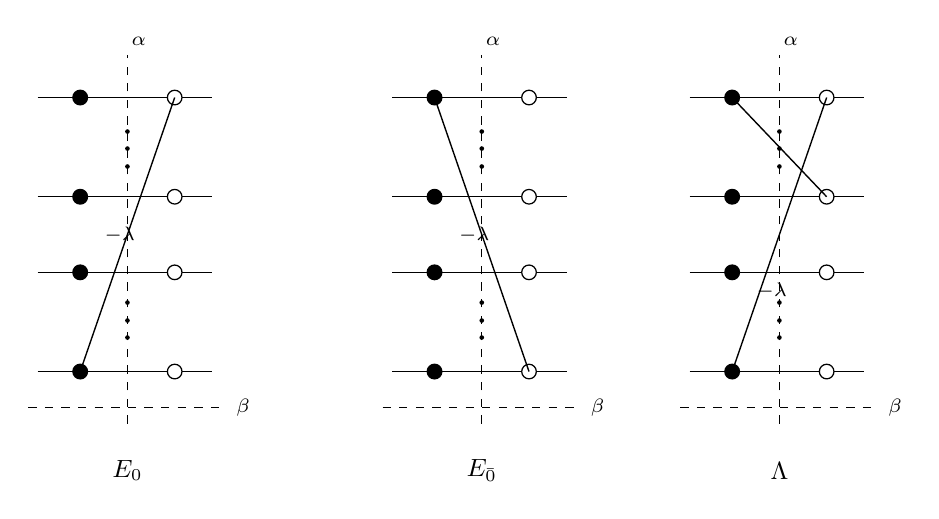
\begin{tikzpicture}[scale=1.20]
\draw[line width=0.5pt] (-0.45,3.00) -- (0.00,3.00);
\draw[line width=0.5pt] (0.00,3.00) -- (1.00,3.00);
\draw[line width=0.5pt] (1.00,3.00) -- (1.40,3.00);
\fill (0.00,3.00) circle (2.4pt);
\fill[white] (1.00,3.00) circle (2.2pt);
\draw[line width=0.45pt] (1.00,3.00) circle (2.2pt);
\draw[line width=0.5pt] (-0.45,1.95) -- (0.00,1.95);
\draw[line width=0.5pt] (0.00,1.95) -- (1.00,1.95);
\draw[line width=0.5pt] (1.00,1.95) -- (1.40,1.95);
\fill (0.00,1.95) circle (2.4pt);
\fill[white] (1.00,1.95) circle (2.2pt);
\draw[line width=0.45pt] (1.00,1.95) circle (2.2pt);
\draw[line width=0.5pt] (-0.45,1.15) -- (0.00,1.15);
\draw[line width=0.5pt] (0.00,1.15) -- (1.00,1.15);
\draw[line width=0.5pt] (1.00,1.15) -- (1.40,1.15);
\fill (0.00,1.15) circle (2.4pt);
\fill[white] (1.00,1.15) circle (2.2pt);
\draw[line width=0.45pt] (1.00,1.15) circle (2.2pt);
\draw[line width=0.5pt] (-0.45,0.10) -- (0.00,0.10);
\draw[line width=0.5pt] (0.00,0.10) -- (1.00,0.10);
\draw[line width=0.5pt] (1.00,0.10) -- (1.40,0.10);
\fill (0.00,0.10) circle (2.4pt);
\fill[white] (1.00,0.10) circle (2.2pt);
\draw[line width=0.45pt] (1.00,0.10) circle (2.2pt);
\fill (0.50,2.64) circle (0.7pt);
\fill (0.50,2.46) circle (0.7pt);
\fill (0.50,2.27) circle (0.7pt);
\fill (0.50,0.83) circle (0.7pt);
\fill (0.50,0.64) circle (0.7pt);
\fill (0.50,0.46) circle (0.7pt);
\draw[line width=0.5pt] (0.00,0.10) -- (1.00,3.00);
\node[font=\scriptsize] at (0.42,1.55) {$-\lambda$};
\draw[dashed,line width=0.4pt] (0.50,-0.45) -- (0.50,3.45);
\node[font=\scriptsize,above] at (0.62,3.45) {$\alpha$};
\draw[dashed,line width=0.4pt] (-0.55,-0.28) -- (1.55,-0.28);
\node[font=\scriptsize,right] at (1.55,-0.28) {$\beta$};
\node[font=\small] at (0.50,-0.95) {$E_0$};
\begin{scope}[xshift=3.75cm]
\draw[line width=0.5pt] (-0.45,3.00) -- (0.00,3.00);
\draw[line width=0.5pt] (0.00,3.00) -- (1.00,3.00);
\draw[line width=0.5pt] (1.00,3.00) -- (1.40,3.00);
\fill (0.00,3.00) circle (2.4pt);
\fill[white] (1.00,3.00) circle (2.2pt);
\draw[line width=0.45pt] (1.00,3.00) circle (2.2pt);
\draw[line width=0.5pt] (-0.45,1.95) -- (0.00,1.95);
\draw[line width=0.5pt] (0.00,1.95) -- (1.00,1.95);
\draw[line width=0.5pt] (1.00,1.95) -- (1.40,1.95);
\fill (0.00,1.95) circle (2.4pt);
\fill[white] (1.00,1.95) circle (2.2pt);
\draw[line width=0.45pt] (1.00,1.95) circle (2.2pt);
\draw[line width=0.5pt] (-0.45,1.15) -- (0.00,1.15);
\draw[line width=0.5pt] (0.00,1.15) -- (1.00,1.15);
\draw[line width=0.5pt] (1.00,1.15) -- (1.40,1.15);
\fill (0.00,1.15) circle (2.4pt);
\fill[white] (1.00,1.15) circle (2.2pt);
\draw[line width=0.45pt] (1.00,1.15) circle (2.2pt);
\draw[line width=0.5pt] (-0.45,0.10) -- (0.00,0.10);
\draw[line width=0.5pt] (0.00,0.10) -- (1.00,0.10);
\draw[line width=0.5pt] (1.00,0.10) -- (1.40,0.10);
\fill (0.00,0.10) circle (2.4pt);
\fill[white] (1.00,0.10) circle (2.2pt);
\draw[line width=0.45pt] (1.00,0.10) circle (2.2pt);
\fill (0.50,2.64) circle (0.7pt);
\fill (0.50,2.46) circle (0.7pt);
\fill (0.50,2.27) circle (0.7pt);
\fill (0.50,0.83) circle (0.7pt);
\fill (0.50,0.64) circle (0.7pt);
\fill (0.50,0.46) circle (0.7pt);
\draw[line width=0.5pt] (0.00,3.00) -- (1.00,0.10);
\node[font=\scriptsize] at (0.42,1.55) {$-\lambda$};
\draw[dashed,line width=0.4pt] (0.50,-0.45) -- (0.50,3.45);
\node[font=\scriptsize,above] at (0.62,3.45) {$\alpha$};
\draw[dashed,line width=0.4pt] (-0.55,-0.28) -- (1.55,-0.28);
\node[font=\scriptsize,right] at (1.55,-0.28) {$\beta$};
\node[font=\small] at (0.50,-0.95) {$E_{\bar0}$};
\end{scope}
\begin{scope}[xshift=6.90cm]
\draw[line width=0.5pt] (-0.45,3.00) -- (0.00,3.00);
\draw[line width=0.5pt] (0.00,3.00) -- (1.00,3.00);
\draw[line width=0.5pt] (1.00,3.00) -- (1.40,3.00);
\fill (0.00,3.00) circle (2.4pt);
\fill[white] (1.00,3.00) circle (2.2pt);
\draw[line width=0.45pt] (1.00,3.00) circle (2.2pt);
\draw[line width=0.5pt] (-0.45,1.95) -- (0.00,1.95);
\draw[line width=0.5pt] (0.00,1.95) -- (1.00,1.95);
\draw[line width=0.5pt] (1.00,1.95) -- (1.40,1.95);
\fill (0.00,1.95) circle (2.4pt);
\fill[white] (1.00,1.95) circle (2.2pt);
\draw[line width=0.45pt] (1.00,1.95) circle (2.2pt);
\draw[line width=0.5pt] (-0.45,1.15) -- (0.00,1.15);
\draw[line width=0.5pt] (0.00,1.15) -- (1.00,1.15);
\draw[line width=0.5pt] (1.00,1.15) -- (1.40,1.15);
\fill (0.00,1.15) circle (2.4pt);
\fill[white] (1.00,1.15) circle (2.2pt);
\draw[line width=0.45pt] (1.00,1.15) circle (2.2pt);
\draw[line width=0.5pt] (-0.45,0.10) -- (0.00,0.10);
\draw[line width=0.5pt] (0.00,0.10) -- (1.00,0.10);
\draw[line width=0.5pt] (1.00,0.10) -- (1.40,0.10);
\fill (0.00,0.10) circle (2.4pt);
\fill[white] (1.00,0.10) circle (2.2pt);
\draw[line width=0.45pt] (1.00,0.10) circle (2.2pt);
\fill (0.50,2.64) circle (0.7pt);
\fill (0.50,2.46) circle (0.7pt);
\fill (0.50,2.27) circle (0.7pt);
\fill (0.50,0.83) circle (0.7pt);
\fill (0.50,0.64) circle (0.7pt);
\fill (0.50,0.46) circle (0.7pt);
\draw[line width=0.5pt] (0.00,3.00) -- (1.00,1.95);
\draw[line width=0.5pt] (0.00,0.10) -- (1.00,3.00);
\node[font=\scriptsize] at (0.42,0.95) {$-\lambda$};
\draw[dashed,line width=0.4pt] (0.50,-0.45) -- (0.50,3.45);
\node[font=\scriptsize,above] at (0.62,3.45) {$\alpha$};
\draw[dashed,line width=0.4pt] (-0.55,-0.28) -- (1.55,-0.28);
\node[font=\scriptsize,right] at (1.55,-0.28) {$\beta$};
\node[font=\small] at (0.50,-0.95) {$\Lambda$};
\end{scope}
\end{tikzpicture}
\caption{对应于 $\widehat{\operatorname{PGL}}(N)$ 的依赖于谱参数的生成元的图。虚线仍表示圈 $\alpha$（竖直）与 $\beta$（水平）。现在对 $\lambda$-相关子式有 $\langle\beta,D\rangle=1$，相应的 $Q(D)=\langle\alpha,D\rangle\langle\beta,D\rangle=\langle\alpha,D\rangle$ 计算被占据的终止边的条数。}
\label{fig:1.8}
\end{figure}

\subsection{对偶曲面、双重配分函数与 Poisson 括号}

回忆：图到可定向曲面的嵌入诱导一个\emph{厚图}结构，即每个顶点处关联边端点的循环次序。反之，给定厚图结构，存在唯一（模微分同胚）的曲面与嵌入，诱导基本群的满射。依 [11]，我们引入二部图到两个曲面的\emph{对偶嵌入}概念。两个嵌入 $\Gamma\to\Sigma$ 与 $\Gamma\to\tilde\Sigma$ 称为对偶的，如果二者都诱导基本群的满射，且两个嵌入诱导的厚图结构在白顶点处相同、在黑顶点处相反。

对偶曲面 $\tilde\Sigma$ 也可以如下想象。$\Gamma$ 上的\emph{之字形路径}是在每个白顶点处左转、在每个黑顶点处右转的路径。沿每条之字形路径给图 $\Gamma$ 粘上一个圆盘。由于 $\Gamma$ 的每条边恰属于两条之字形路径，我们得到闭光滑曲面 $\tilde\Sigma$。之字形路径是对偶曲面 $\tilde\Sigma$ 的面的边界，但它在 $\Sigma$ 的同调中可能非平凡。反之，$\Sigma$ 的面的边界在 $\tilde\Sigma$ 中可能不可收缩。之字形路径在同调 $H_1(\Sigma)$ 中的和显然为零，因此它们是 $H_1(\Sigma,\R)$ 中一个顶点在整点的凸多边形 $\Delta$ 的边。多边形 $\Delta$ 定义到平移为止。

注意此时在同调层面有显然的映射：
\[
i: H_1(\Gamma)\to H_1(\Sigma),\qquad
\tilde\imath: H_1(\Gamma)\to H_1(\tilde\Sigma),\qquad
i^*: H_1(\Sigma)\to H_1(\Gamma),\qquad
\tilde\imath^*: H_1(\Gamma)\to H_1(\tilde\Sigma).
\]
如 [11] 所证明，若图 $\Gamma$ 极小，则映射 $i+\tilde\imath$ 的余核 $Z$ 有限，因此映射 $i^*\times\tilde\imath^*$ 的核 $Z^*$ 也有限。

记 $C_1\subset H_1(\Gamma)$ 为 $i+\tilde\imath$ 的核，$C^1$ 为 $i^*\times\tilde\imath^*$ 的余核。固定正合列
\begin{equation}\label{eq:1.33}
1\to Z^*\to H_1(\Sigma)\times H_1(\tilde\Sigma)\to H_1(\Gamma)\to C^1\to1
\tag{1.33}
\end{equation}
的分裂，可以构造映射 $\bar A: H_1(\Sigma)\times H_1(\tilde\Sigma)\times C_1\to C^1(\Gamma)$，从而得到配分函数的又一个版本，我们称之为\emph{双重配分函数} $S^d_\Gamma(\lambda,\tilde\lambda,c)=S_\Gamma(\bar A(\lambda,\tilde\lambda,c))$。这个双重配分函数依赖于分裂，因此定义到变换
\[
S^d_\Gamma(\lambda,\tilde\lambda,c)\mapsto\alpha(c)S^f_\Gamma(\beta(c)\lambda,\tilde\beta(c)\tilde\lambda,c)
\]
为止，其中 $\alpha: C_1\to\C^\times$、$\beta: C_1\to H_1(\Sigma)$、$\tilde\beta: C_1\to H_1(\tilde\Sigma)$ 是任意同态。

注意序列 (1.33) 蕴涵空间 $B^2(\Sigma)$ 同构于 $(H_1(\tilde\Sigma)\times C_1)/Z^*$。确实，这个同构由微分 $\partial: H_1(\tilde\Sigma)\times C_1\to B^2(\Sigma)$ 给出。

回忆空间 $H_1(\tilde\Sigma)$ 带有典范 Poisson 括号，来源于 $H_1(\tilde\Sigma)$ 上的相交指数 $\langle\cdot,\cdot\rangle_{\tilde\Sigma}$。确实，对由整同调类 $x,y\in H_1(\tilde\Sigma)$ 定义在 $H_1(\tilde\Sigma)$ 上的两个函数 $\langle\cdot,x\rangle$ 与 $\langle\cdot,y\rangle$，括号由
\begin{equation}\label{eq:1.34}
\{\langle\cdot,x\rangle,\langle\cdot,y\rangle\}=\langle x,y\rangle\langle\cdot,x+y\rangle
\tag{1.34}
\end{equation}
给出，其中 $x$ 与 $y$ 之间的配对是相交指数\footnote{对 $H_1(\tilde\Sigma)$ 中的典范 $A$-圈与 $B$-圈（其选择使 $\langle A_i,B_j\rangle=\delta_{ij}$）对偶的函数，可以扮演（指数化）坐标与动量的角色。}。这个括号显然在乘法平移下不变，特别地在有限群 $Z^*$ 的作用下不变。于是乘积 $H_1(\tilde\Sigma)\times C_1$ 在第二个因子上有平凡 Poisson 结构，而映射 $\partial$ 在 $B^2(\Sigma)$ 上诱导一个。

现在回忆空间 $B^2(\Sigma)$ 有自然的坐标，由给嵌入 $\Sigma$ 的 $\Gamma$ 的面赋数给出。在这些坐标下括号 (1.34) 由组合公式（与附录 1.9 中的括号 (1.57) 比较）
\begin{equation}\label{eq:1.35}
\{x_i,x_j\}=\varepsilon_{ij}x_ix_j
\tag{1.35}
\end{equation}
给出。这里 $i,j\in B^2(\Sigma)$ 是两个面，$\varepsilon_{ij}$ 是公共边的条数，从 $i$ 走到 $j$ 时若白顶点在右侧则取正号，否则取负号。换言之，Poisson 括号 (1.34)、(1.35) 的交换图恰是图 $\Gamma$ 的对偶。
